%! TEX root = ./master.tex
\lecture[Beispiele zu Seifert van Kampen. $k$-Zellen. CW-Komplexe. Realisierung von Sphären, Tori und  $\R\mathbb{P}^n$ als CW-Komplexe.]{Di 06 Jul 2021 12:13}{CW-Komplexe}

\begin{orga}
    Es gibt jetzt mehr Infos zur Klausur. Dazu findet sich auf eCampus ein Merkblatt zur Klausur. Das wichtigste ist vor allem, eine Ausweiskopie vorher einzusenden.
\end{orga}

\section{Der Satz von Seifert von Kampen und CW-Komplexe}

\begin{restatable}[Seifert-van-Kampen]{theorem}{ThmSeifertVanKampen}\label{thm:seifert-van-kampen}
    Sei $X$ ein Raum, seien  $U_1,U_2\subset X$ offen, sodass $U_1\cup U_2 = X$, und bezeichne  $U_3 \coloneqq  U_1 \cap U_2$.

    Sind $U_1,U_2,U_3$ wegzusammenhängend und nicht-leer sowie $x_0\in U_3$, dann ist
    \[
        \begin{tikzcd}[ampersand replacement = \&]
        \pi_1(U_3,x_0) \ar[swap]{d}{} \ar{r}{} \& \pi_1(U_1,x_0) \ar{d}{} \\
        \pi_1(U_2,x_0) \ar[swap]{r}{} \& \pi_1(X,x_0)
    \end{tikzcd}
    l\]
    ein Pushout von Gruppen, d.h. für jede Gruppe $H$ und kompatible Morphismen  $\pi_1(U_1,x_0) \to  H$ sowie $\pi_1(U_2,x_0) \to  H$ existiert ein eindeutig bestimmter Morphismus $\pi_1(X,x_0) \to  H$. Visualisiert:
    \[
        \begin{tikzcd}[ampersand replacement = \&]
        \pi_1(U_3,x_0) \ar[swap]{d}{} \ar{r}{} \& \pi_1(U_1,x_0) \ar{d}{} \\
        \pi_1(U_2,x_0) \ar[swap]{r}{} \& \pi_1(X,x_0)
    \end{tikzcd}
    \]
\end{restatable}

\begin{figure}[ht]
    \centering
    \incfig{skizze-zu-seifert-van-kampen}
    \caption{Skizze zu Seifert van Kampen}
    \label{fig:skizze-zu-seifert-van-kampen}
\end{figure}

Betrachte Abbildung \ref{fig:skizze-zu-seifert-van-kampen}, da 'sieht man' viel zur Intuition von Seifert van Kampen.


Wir erinnerns uns hier auch noch an \autoref{def:wedge-produkt}, das letztendlich auch nur ein Pushout von Räumen ist. Wir können also Seifert van Kampen auch umformulieren zu 'Seifert van Kampen erhält \textit{schöne} Pushouts'.

Wir können diese Intuition nun in einer kombinatorischer Form ausdrücken, hierzu sei $x_0\in U_3 \coloneqq  U_2 \cap U_1$ mit $U_1 \cup U_2 = X $ gegeben. Mit $\pi_1$ erhalten wir bereits ein Diagramm
\[
\begin{tikzcd}
    \pi_1(U_3, x_0)\ar[swap]{d}{\varphi_2 } \ar{r}{\varphi_1} & \pi_1(U_1,x_0) \\
    \pi_1(U_2,x_0)
\end{tikzcd}
\]

Wählen wir nun Gruppendarstellungen

\begin{IEEEeqnarray*}{rCl}
    \pi_1(U_1,x_0) & \cong & \left< α_1, \ldots, α_k \mid  r_1, \ldots, r_l \right> \\
    \pi_1(U_2,x_0) & \cong & \left< β_1, \ldots, β_m \mid  s_1, \ldots, s_n\right>  \\
    \pi_1(U_3,x_0) & \cong & \left< γ_1, \ldots, γ_p \mid  t_1, .., t_q \right> 
\end{IEEEeqnarray*}



\begin{corollary}\label{cor:seifert-van-kampen-für-einfach-zusammenhängende-räume}
    Sei $X = U_1 \cup U_2$, $U_3 \coloneqq  U_1 \cap  U_2$ mit $U_i$ offen und wegzusammenhängend sowie nichtleer. Sind  $U_1,U_2$ einfach zusammenhängend, so ist $\pi_1(X) = 1$.
\end{corollary}

\begin{example}
    Es ist $\pi_1(S^n) = 1$ für $n\geq 2$. Das haben wir schon einmal 'von Hand' gezeigt, mit \autoref{fig:skizze-zu-seifert-van-kampen} ist das aber sehr einfach:

    Betrachte wieder $N,S$ als den Nord- und Südpol von  $S^n$, und setze  $U_1 \coloneqq  S^n \setminus N\cong \R^n$, $U_2 \coloneqq  S^n \setminus S \cong \R^n$ (wir erinnerns uns an die stereographische Projektion).

    Dann ist sicherlich $S^n = U_1 \cup U_2$, und wir erhalten auch
    \[
        U_3 \coloneqq  U_1 \cap  U_2 = S^n \setminus \left \{N,S\right\} \cong S^{n-1} \times (-1,1)
    .\] 
    Wegen $n\geq 2$ ist das nun wegzusammenhängend. Mit \autoref{cor:seifert-van-kampen-für-einfach-zusammenhängende-räume} erhalten wir dann sofort, dass $\pi_1(S^n) = 1$.

    Man könnte auch direkt \autoref{thm:seifert-van-kampen} verwenden, dann ergibt sich
    \[
        \pi_1(S^n) \cong \pi_1(U_1) \star_{\pi_1(U_3)} \pi_1(U_2) = 1 \star 1 = 1
    .\] 
    \begin{oral}
        Man köme in Versuchung, einfach für $U_1,U_2$ die obere und untere Halbkugel zu verwenden, dann ist der Schnitt - der Äquator - ebenfalls wegzusammenhängend. Das darf man aber im allgemeinen nicht machen, wir brauchen wirklich, dass $U_1,U_2$ offen sind. Dass die Anwendung hier funktioniert, ist nur 'Zufall'.
    \end{oral}
    \begin{warning}
        Der Beweis gilt nicht für $S^1$, da  $U_3 \cong S^0 \times  (-1,1)$, da $S^0$ \textit{nicht} wegzusammenhängend ist.
    \end{warning}
\end{example}

\begin{example}
    Betrachte zwei Kopien des Torus, und identifiziere sie entlang einer Schleife.
    \missingfigure{Torus 'in' Torus verklebt}
    Formal definieren wir $X$ durch
     \[
         X\coloneqq \faktor{S^1 \times  S^1 \times \left \{1\right\} \sqcup S^1 \times S^1 \times  \left \{2\right\} }{S^1 \times \left \{1\right\} \times \left \{1\right\} \sim  S^1 \times \left \{1\right\} \times \left \{2\right\} }
    .\] 
    Wir würden jetzt gerne $T_1,T_2$ (die Tori) in $X$ verwenden und \nameref{thm:seifert-van-kampen} anwenden, aber diese sind nicht offen. Wir müssen die Tori also 'etwas' vergrößern, sodass sie offen sind, ohne dass wir die schönen Eigenschaften der Tori verlieren. Man gelangt zu:
    \begin{IEEEeqnarray*}{rCl}
        A_1 &\coloneqq&  S^1 \times (e^{-i\theta}, e^{i\theta}) \subset T_1 \\
        A_2        & \coloneqq  & S^1 \times  (e^{-i\theta}, e^{i\theta}) \subset T_2 \\
        U_1 & \coloneqq  & T_1 \cup A_2  \simeq T_1\\
        U_2 &\coloneqq & T_2 \cup A_1 \simeq T_2
    \end{IEEEeqnarray*}
    Die Homotopieäquivalenz erhalten wir einfach durch stetiges zusammenziehen dieses 'angeklebten' Schlauches $A_i$.

    Jetzt sind also  $U_1,U_2$ offen und verhalten sich wie unsere Tori, und der Schnitt ergibt sich als $U_3 \coloneqq  U_1 \cap  U_2 = A_1 \cup A_2$, und dieser ist auch wegzusammenhängend.

    Also ergibt sich nun mit \nameref{thm:seifert-van-kampen}, dass
    \[
        \pi_1(X) \cong \pi_1(U_1,x ) \star_{\pi_1(U_3,x)} \pi_1(U_2, x) 
    .\] 

Da wir schon wissen, dass $\pi_1(T_1) \cong \Z \times  \Z$ die Fundamentalgruppe des Torus ist, und das lässt sich darstellen als
\begin{IEEEeqnarray*}{rCl}
    \pi_1(T_1) & = & \left< a,b \mid  ab a^{-1} b^{-1} \right> \\
    \pi_1(T_2)               & = & \left< c,d \mid  cdc^{-1}d^{-1} \right> 
\end{IEEEeqnarray*}
Man überlegt sich noch, dass $U_3 = A_1 \cup A_2 \simeq S^1$, auch indem wir die extra 'Schläuche' stetig verkürzen, also $\pi_1(U_3) = \Z = \left< γ \mid  \right> $.
\begin{IEEEeqnarray*}{rCl}
    \pi_1(X,x) & = & \left< a,b,c,d \mid  aba^{-1}b^{-1}, cdc^{-1}d^{-1}, a  =  c \right> \\
                                                                            & = & \left< a,b,c,d \mid aba^{-1}b^{-1}, cdc^{-1}d^{-1}, ac^{-1} \right> 
\end{IEEEeqnarray*}
\begin{oral}
    Man kann auch eine andere Darstellung von $X$ wählen, indem wir die 'lange' Schleife von  $X$ wählen (die in Wahrheit aber natürlich Symmetrisch ist). Dann kann man sich  $X$ als 'Stapel von Donuts' vorstellen, die einfach übereinander liegen und sich kanonisch berühren. Dann sieht man auch, dass
     \[
         X = (S^1 \twedge S^1 ) \times S^1
    .\] 
    und wir würden schnell erhalten, dass
    \begin{IEEEeqnarray*}{rCl}
        \pi_1(X) & = & \pi_1(S^1 \twedge S^1) \times  \pi(S^1) \\
                 & = & \left< b,d\mid  \right> \times \left< a\mid  \right> \\
                 & = & \left< a,b,d\mid aba^{-1}b^{-1}, ada^{-1}d^{-1} \right> 
    \end{IEEEeqnarray*}
    Man sieht auch leicht, dass die beiden Darstellungen, die wir erhalten haben, die gleichen Gruppen beschreiben.
\end{oral}
\end{example}

\begin{dnotation}[Freie Gruppen]
    Die Notation $\left< a \mid  \right> $ heißt natürlich, dass wir keine Relationen fordern, also $\left<  a \mid  \right>  \cong \Z$. Manchmal lässt man diesen Strich dann auch weg, und schreibt einfach sofort
    \[
    \left< a \right>  \cong \Z
    .\] 
    Das darf man aber nicht verwechseln mit der von $g$ erzeugten Untergruppe, wenn  $g\in G$ bereits ein Element ist, hier erhalten wir natürlich implizit alle Relationen, die $g$ als Element von $G$ besitzt.
\end{dnotation}

\begin{definition}[$k$-Zelle]\label{def:k-zelle}
    Eine \vocab{$k$-Zelle},  $k\geq 0$, ist ein Raum der homöomorph zu $D^k$ ist. Eine \vocab{offene $k$-Zelle} ist eine ein Raum, der homöomorph zu ${D^k}\degree$  ist, wobei wie üblich
    \[
        D^k \coloneqq  \left \{(x,\ldots,x_k) \mid  \sum x_i ^2 \leq  1\right\} \\
        {D^k}\degree \coloneqq  \left \{(x_1,\ldots,x_k) \mid  \sum x_i^2 < 1\right\} 
    .\] 
    Wir nenen $k$ die  \vocab{Dimension} der Zelle. 
\end{definition}

\begin{definition}{CW-Komplex}\label{def:cw-komplex}
    Ein CW-Komplex  $X$ ist ein Hausdorff-Raum, der in offene Zellen  $\left \{c_i\right\} _{i \in I}$ zerfällt, wobei gilt:
    \begin{enumerate}[1.]
        \item Zu jeder $k$-Zelle  $c_i \subset X$ existiert eine stetige Abbildung $f_i \colon  D^k \to  X$, sodass ${D^k}\degree \subset D^k$ homöomorph auf $c_i$ und der Rand  $\partial D^k = S^{k-1} \subset D^k$ in eine Vereinigung von endlich vielen Zellen der Dimension $<k$ abgebildet wird. 
        \item $M\subset X$ ist genau dann offen, wenn $M \cap f_i(D^k)$ für alle $i\in I$ offen ist.
    \end{enumerate}
\end{definition}

\begin{oral}
    $C$ stet für 'closure finite', und  $W$ steht für 'weak'.
\end{oral}

\begin{dnotation}
    Das \vocab{k}-Gerüst oder auch \vocab{k}-Skeleet von $X$, notiert  $X^k$, ist die Vereinigung aller seiner Zellen der Dimension  $\leq k$.  
\end{dnotation}

\begin{remark}
    Jeder CW-Komplex ist normal (und Hausdorff) sowie lokal zusammenziehbar, d.h. jeder Punkt besitzt eine zusammenziehbare Umgebung.

    Insbesondere ist jeder CW-Komplex
    \begin{itemize}
        \item lokal wegzusammenhängend
        \item (semi) lokal einfachzusammenhängend
    \end{itemize}
    und damit besitzt er eine universelle Überlagerung.
\end{remark}


\begin{question}
    Wie bildet man einen CW-Komplex?
\end{question}

Meistens erfolgt das mit einer induktiven / rekursiven Konstruktion, indem wir nacheinander die $k$-Skelette spezifizieren. Wir starten mit 
 \begin{enumerate}[1.]
     \item $X^0$, das  $0$-Gerüst, ist ein diskreter Raum (Punkte sind  $0$-Zellen).
     \item Haben wir das $k$-Gerüst $X^k$, $k\geq 0$ bereits gegebn, und eine Abbildung
         \[
         \varphi _{α}\colon  \partial D^{k+1} = S^k \longrightarrow  X^k
         .\] 
         so können wir eine $k+1$-Zelle an  $X^k$ 'ankleben'. Dazu betrachte
          \[
\faktor{X^k \bigsqcup D^{k+1}}{x \sim  \varphi _{α}(x)} =: X^k \cup_{\varphi _{α}} D^{k+1}
         .\] 
         so setzen wir
         \[
             X^{k+1} \coloneqq  X^k \cup _{\left \{\varphi _{α}\right\} } (D^{k+1})_{α}
         .\] 
         indem wir alle $k+1$-Zellen gleichzeitig ankleben.
\end{enumerate}

\begin{remark}
    Für endliche CW-Komplexe stimmen die Quotiententopologie und die schwache Topologie überein.
\end{remark}

\begin{oral}
    Für unendliche Räume erhalten wir genau die Koprodukttopologie.
\end{oral}

\begin{oral}
    Der Hawaiianische Ohrring ist kein CW-Komplex.
\end{oral}

\begin{notation*}
    Ist $X$ ein CW-Komplex, und existiert  $N$, sodass  $X = X^N$ mit  $N$ minimal, so heißt  $N$ die  \vocab{Dimension} von $X$. 
\end{notation*}

\begin{example}
    Ein 1-dimensionaler CW-Komplex heißt auch \vocab{Graph}. Er besteht aus 0-Zellen und 1-Zellen. Die 0-Zellen nennen wir \vocab{Ecken} oder auch \vocab{Knoten}, die 1-Zellen \vocab{Kanten}.
\[
    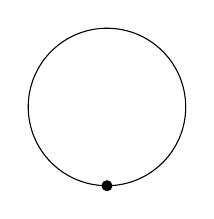
\begin{tikzpicture}
        \draw (0,0) circle (1);
        \fill (0,-1) circle (2pt);
    \end{tikzpicture}
\]
\missingfigure{Graph}
\begin{oral}
    \begin{warning}
        Man muss aufpassen, was passiert, wenn es unendlich viele Kanten in einem Punkt gib.
    \end{warning}
\end{oral}
\end{example}

\begin{example}[zwei-dimensional]
    Die Sphäre kann auch als CW-Komplex realisiert werden, indem wir eine 0-Zelle und eine 2-Zelle verwenden. Starten wir mit einem Punkt, so gibt es eine offensichtliche Abbildung $\partial D^2 \to  X^0 = \left \{S\right\} $. Wir kleben dann einfach den Rand von $D^2$ an den Punkt und erhalten sofort die Kugel.

    Alternativ kann man $S^n$ auch induktiv aufbauen, indem wir verwenden, dass  $S^n$ der Äquator von  $S^{n+1}$ ist, und dann jeweils 2 $n+1$-Zellen an  $S^n$ kleben, um  $S^{n+1}$ zu erhalten.

    Schauen wir nun auf $\R\mathbb{P}^n \coloneqq  \faktor{S^n}{x \sim -x}$, so sehen wir, dass wir die beiden Zellen, die wir für $S^n$ bekommen haben, jeweils identifizieren. Wir können  $\R\mathbb{P}^n$ also realisieren als CW-Komplex mit einer 0, einer 1, \ldots, und einer $n$-Zelle.

    Ein weiterer toller Punkt dieser auf den ersten Blick aufwendigeren Zellstruktur für  $S^n $ ist, dass wir nun
    \[
    S^{\infty} \coloneqq  \bigcup_{k=0}^{\infty} S^k 
    .\] 
    als die unendlich-dimensionale Sphäre als CW-Komplex definiert / realisiert haben.

    Der Torus kann ebenfalls so realisiert werden, hierzu benötigen wir eine 0-Zelle, zwei 1-Zellen sowie eine 2-Zelle.

    Erinnern wir uns an $\R\mathbb{P}^2 \coloneqq  \faktor{S^2}{x \sim  -x} \cong \faktor{D^2}{x \sim  -x \text{ für }x \in \partial D^2}$. Damit erhalten wir wieder eine Darstellung von $\R\mathbb{P}^2$ als eine 0, eine 1 und eine 2-Zelle.
\end{example}
